\section{OpenCL}
\label{sec:opencl}

\subsection{Einleitung}

In diesem Abschnitt wird OpenCL als das Framework, welches für die Berechnungen
verwendet wurde, vorgestellt. Dabei wird im ersten Teil zunächst eine kurzer
geschichtlicher Abriss gegeben und die Stellung von OpenCL unter anderen
Frameworks herausgestellt. Im Anschluss wird der Begriff Parallelität definiert
und speziellere Ausprägungen davon im Kontext mit OpenCL besprochen. Mit diesem
Wissen lässt sich abschätzen, wieso die vorgestellten Algorithmen sich besonders
für eine parallele Abarbeitung eignen.

Im nächsten Abschnitt wird die Architektur von OpenCL im Detail vorgestellt,
wobei für die für die Arbeit irrelevanten Teile nur angeschnitten werden.

Schließlich wird ein vollständiges Programm vorgestellt, welches eine einfache
Berechnung in OpenCL durchführt. Dies soll vor allem den in der Implementierung
immer wiederkehrenden Arbeitsablauf deutlich machen, der nötig ist, um Daten und
Programme auf der GPU zu verwalten. Im Kapitel über die konkret implementierten
Algorithmen wird dann nur noch der OpenCL-C-Code beschrieben.

\subsection{Geschichtliches}

Strömungsmechanische Berechnungen gelten als sehr rechenaufwändiges
Problem, für das traditionell große Rechencluster eingesetzt werden.
Diese Cluster bestehen üblicherweise aus tausenden einzelnen
Prozessoren, die jeweils einen kleinen Teil des Problems lösen, zum
Beispiel nur einen Ausschnitt des Definitionsbereichs berechnen. Alle
Prozessoren werden zu einem 3D-Gitter zusammengefasst und decken so
den gesamten Simulationsbereich ab. Dadurch, dass die Recheneinheiten
parallel arbeiten können, erhält man schnell eine Lösung des Problems.

Desktop-Rechner hatten bis vor einigen Jahren allerdings nur einen
einzelnen Prozessor zum Rechnen verbaut, sodass die oben beschriebene
Arbeitsweise nicht übertragbar war. Tatsächlich zeigte sich bei
Desktop-CPUs bis ca.\,2005 ein Anstieg in der Taktrate der
Prozessoren, aber nicht deren Anzahl\PimiddyTodo{Tabelle mit Anstieg
der Taktrate einbauen}. Diese Entwicklung endete allerdings, da mit
der Taktrate auch der Stromverbrauch immer weiter ansteigt. In
\cite{Chandrakasan1995} findet sich der folgende Zusammenhang zwischen
dem Stromverbrauch in Watt $P$, der Taktfrequenz $f$, der Spannung $V$ und
des Widerstands $C$ eines Prozessors:

\begin{align}
P = C V^2 f
\end{align}

Ersetzt man einen einzelnen Prozessor mit Taktfrequenz $f$, Spannung
$V$ und Widerstand $C$ durch zwei Prozessoren halber Frequenz $f/2$,
so erhöht sich laut \cite{Chandrakasan1995} zwar der Widerstand auf
$2.2C$, aber die Spannung sinkt drastisch auf $0.6V$. Die zwei
Prozessoren verbrauchen daher zusammen nur 0.396 mal so viel Leistung
wie der einzelne Prozessor. Aufgrund dessen geht aktuell der Trend hin
zu Prozessoren mit mehreren Kernen (momentan bis zu 8).

In den letzten Jahren ist auch die Leistungsfähigkeit von
Grafikprozessoren (GPUs) rasant angestiegen (siehe
\autoref{fig:opencl_gflops_gpu_vs_cpu} und
\autoref{fig:opencl_gbs_gpu_vs_cpu}). GPUs waren anfangs spezialisierte Recheneinheiten, um die in
\autoref{sec:opengl} vorgestellte Grafikpipeline umzusetzen. Da jeder
Vertex und jedes Fragment für sich bearbeitet werden kann, bot sich
hier von Anfang an eine hochparallele Architektur an.

\begin{figure}
	\begin{subfigure}[t]{0.5\textwidth}
		\centering
		\includegraphics[width=\textwidth]{images/gflops_cpu_vs_gpu}
                \caption{Anstieg der Gigaflops pro Sekunde im Vergleich zwischen CPUs und GPUs}
		\label{fig:opencl_gflops_gpu_vs_cpu}
	\end{subfigure}
	~
	\begin{subfigure}[t]{0.5\textwidth}
		\centering
		\includegraphics[width=\textwidth]{images/gbs_cpu_vs_gpu}
                \caption{Anstieg der Bandbreite im Vergleich zwischen CPUs und GPUs}
		\label{fig:opencl_gbs_gpu_vs_cpu}
	\end{subfigure}
        \caption{Vergleich zwischen CPUs und GPUs}
\end{figure}

Mit der Zeit stieg aber die Nachfrage nach mächtigeren Shaderprogrammen, um
aufwändigere Grafikeffekte umzusetzen. Daher wurden die Recheneinheiten der GPUs
immer weiter verallgemeinert. Mit Hilfe dieser leistungsfähigen Shaderprogramme
begannen auch Wissenschaftler, Grafikkarten für Rechenaufgaben zu verwenden und
es entstanden \Pimiddyca 2004 erste Umsetzungen von Stams Methode auf
Grafikkarten\cite{Wu2004}.

Allerdings war es bis dato weder möglich, rohen Speicher auf der
Grafikkarte zu reservieren, noch beliebige Programme zu starten, die
auf diesem Speicher arbeiten. Vielmehr mussten die bestehenden
Mechanismen der Grafikpipeline \PimiddyQuotes{missbraucht} werden. So
wurden Simulationsergebnisse in zweidimensionalen Texturen
gespeichert, die man als \PimiddyQuotes{Rendertargets} angeben
konnte. Dann wurde ein Rechteck auf den Bildschirm gezeichnet, um die
Ausführung der Berechnungs-Shader künstlich anzustoßen.

Um komfortabler allgemeine Berechnungen auf der Grafikkarte bzw. auf
Mehrkernsystemen zu tätigen, wurden mehrere Frameworks entwickelt,
unter anderem CUDA von NVidia und AMDs Stream Framework. Diese waren
aber nicht formal spezifiziert und oft herstellerabhängig. Ein
CUDA-Programm ist \PimiddyzB nur auf GPUs von NVidia lauffähig.

Als Lösung für dieses Problem wurde Ende 2008 das OpenCL-Framework in
der Version 1.0 veröffentlicht, unterstützt von unter anderem Apple,
NVidia, AMD und IBM. OpenCL ermöglicht das Erstellen von parallel
laufenden Programmen auf GPUs, CPUs und sogar FPGAs. Man spricht
allgemein von \PimiddyBegriff{heterogenen Systemen}. Inzwischen ist
OpenCL bei Version 1.2 angelangt, wobei diese noch nicht von allen
Herstellern unterstützt wird.

\subsection{Arten der Parallelität}

Ob ein Problem mit Hilfe einer Grafikkarte gut lösbar ist, hängt vor allem davon
ab, ob es gut \emph{parallelisierbar} ist. Es soll daher in diesem Abschnitt der
Begriff Parallelität definiert werden. Außerdem sollen die verschiedenen
Ausprägungen von Parallelität, die OpenCL unterstützt, erläutert werden.
Schließlich wird begründet, wieso sich Stams Methode gut für die Berechnung mit
OpenCL eignet.

\emph{Parallelität} oder auch \emph{Nebenläufigkeit} liegt im
Allgemeinen vor, wenn mehrere Operationsströme unabhängig voneinander
in einem Zeitschritt fortschreiten können\cite{munshi2011}. Ein
klassisches Beispiel für nebenläufige Operationsströme bieten
\emph{Threads} in Programmiersprachen wie Java. Während ein Thread
beispielsweise auf Daten von einem Netzwerksocket wartet, kann ein
anderer einen Ladebalken anzeigen. Mit Hilfe von Threads können sowohl
gleiche Bereiche des Codes mehrfach parallel ausgeführt werden
(\PimiddyzB eine bestimmte Funktion mit verschiedenen Eingaben) oder
auch vollkommen verschiedene Bereiche.

In OpenCL werden insgesamt zwei Arten von Parallelität unterschieden:
\PimiddyBegriff{Taskparallelität} und
\PimiddyBegriff{Datenparallelität}. Der Unterschied liegt darin, dass
entweder mehrere \emph{Aufgaben} (Tasks) auf die nebenläufigen
Operationsströme verteilt werden oder mehrere \emph{Datenblöcke}.

Die oben genannten Threads werden meistens für taskparallele Probleme
eingesetzt. Hierbei wird ein Problem in mehrere Aufgaben unterteilt,
die möglichst unabhängig voneinander auf den Recheneinheiten
ausgeführt werden können und eventuell auch unabhängig voneinander
Ergebnisse produzieren. Die Operationsströme und die Eingangsdaten der
verschiedenen parallel laufenden Einheiten sind eventuell sehr
unterschiedlich voneinander.

Bei einem \emph{datenparallelen} Problem hingegen wendet man denselben
Operationsstrom (dasselbe Programm) auf jeweils unterschiedliche
Eingabedaten an. Das einfachste Beispiel für Datenparallelität ist
\emph{Single Instruction Multiple Data} (SIMD), wo das Programm meist aus
einer einzigen Operation besteht. Die Addition zweier Arrays ist
beispielsweise ein Problem, das auf diese Weise lösbar ist. Für jedes
Arrayelement wird ein Prozessor verwendet, der folglich nur Logik für
die Addition zweier Zahlen benötigt. Die nebenläufig arbeitenden
Prozesse beeinflussen sich in diesem Beispiel nicht gegenseitig. Dies
ist aber nicht zwingend für ein datenparalleles Problem, und OpenCL
unterstützt auch Synchronisationsmechanismen. Aufwändigere
datenparallele Probleme enthalten \PimiddyInlineCode{if}-Abfragen und
können so unterschiedliche Ausführungspfade je nach Eingabedaten
nehmen. Diese Art der Parallelität nennt man \emph{Single Program
Multiple Data} (SPMD)\cite{Mattson:2004:PPP:1406956}.

Grafikkarten sind aus historischen Gründen sehr gut für datenparallele
Probleme geeignet, denn die Umsetzung der Grafikpipeline stellt
ebenfalls ein solches Problem dar.

Die Funktionen in Stams Verfahren sind alle datenparallel
gestaltet. Als Eingabe dient immer ein dreidimensionales Vektor- oder
Skalarfeld, bei dem jeder Voxel für sich bearbeitet werden kann (unter
Zuhilfenahme seiner Nachbarschaft im Eingabefeld), wodurch wieder ein
Vektor- bzw. Skalarfeld entsteht. Auch das später vorgestellte
Partikelsystem ist ein datenparalleles Problem, denn jede Schneeflocke
kann für sich bearbeitet werden (Flocken beeinflussen sich nicht
gegenseitig im hier gewählten Modell).

\subsection{Architektur}

Die OpenCL-Architektur ist in 4 Teile geteilt, die nun separat
erläutert werden sollen:

\begin{enumerate}
\item Das \PimiddyBegriff{Platform-Model} bietet eine abstrakte
Beschreibung eines heterogenen Systems. Hier wird der
\PimiddyBegriff{Host} als Steuereinheit sowie die Arten der
Komponenten wie Grafikkarten, CPUs und integrierte Chips definiert.
\item Das \PimiddyBegriff{Execution-Model} beschreibt den Begriff
\PimiddyBegriff{Kernel} als ein Programm, das auf dem Device ausgeführt wird, sowie die
Mechanismen um Kernel zu starten und auszuführen.
\item Das \PimiddyBegriff{Memory-Model} beschreibt die unterschiedlichen Speichertypen, die
OpenCL bereitstellt.
\item \PimiddyBegriff{OpenCL-C} stellt momentan die einzige Sprache
dar, mit der parallele Programme in OpenCL verfasst werden können.
\end{enumerate}

\subsubsection{Platform-Model}

OpenCL soll sowohl auf CPUs als auch auf GPUs und sogar
\PimiddyQuotes{exotischeren} Systemen wie FPGAs eingesetzt
werden. Daher müssen als Basis allgemeine Begriffe zur Beschreibung
von Systemen mit mehreren Prozessoren und Komponenten definiert
werden. Dies geschieht im Platform-Model.

OpenCLs Platform-Model ist in \autoref{fig:opencl_platform_model}
dargestellt. Es ist sehr allgemein gehalten, sodass es sich auf eine
Vielzahl von Hardwaresystemen sinnvoll übertragen lässt. Im Modell
existiert genau einen \PimiddyBegriff{Host}, der mehrere
\PimiddyBegriff{Devices} verwaltet. Ein Device ist zum Beispiel eine
Grafikkarte oder eine CPU. Ein typisches Desktopsystem als Host könnte
beispielsweise drei Devices enthalten: eine CPU und zwei Grafikkarten.

Ein Device hat mehrere \PimiddyBegriff{Compute Units} (CU), die
wiederum \PimiddyBegriff{Processing Elements} (PE) enthalten. Die
eigentlichen Berechnungen finden auf den Processing Elements
statt. Auf einer CU laufen meistens mehrere PE parallel und
kommunizieren gegebenenfalls miteinander über CU-eigenen Speicher und
Synchronisationspunkte. Die Unterscheidung zwischen CU und PE muss auf
Hardware-Ebene allerdings nicht vorhanden sein, sie ist aber dennoch
für das Execution-Model wichtig (siehe unten).

Eine Grafikkarte hingegen besitzt im allgemeinen wesentlich mehr
Compute Units und Processing Elements.

\begin{figure}[ht]
\centering
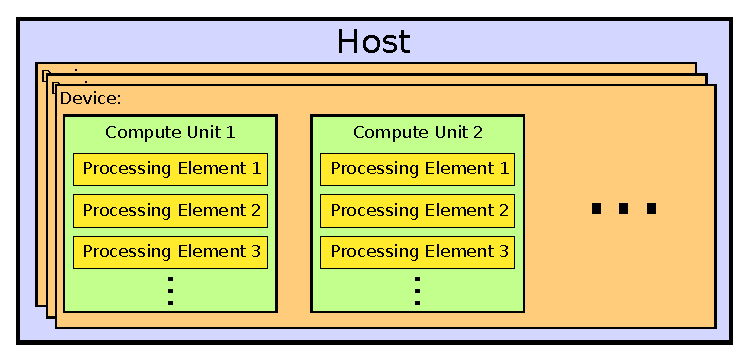
\includegraphics[width=14cm]{images/opencl_platform_model}
\caption{Platform-Model in OpenCL}
\label{fig:opencl_platform_model}
\end{figure}

\subsubsection{Execution-Model}
\label{sec:opencl_execution_model}

Eine OpenCL-Anwendung wird gesteuert durch das Host-Program (das auf
dem Host läuft). Das Host-Programm ist in einer Programmiersprache wie
Java oder C++ geschrieben und ist zuständig für die Reservierung von
Speicher auf den Devices, das Abfragen von Device-Eigenschaften und
dem Starten der sogenannten \PimiddyBegriff{Kernel}.

Kernel sind Programme, die auf dem Device ausgeführt werden und somit
die eigentliche parallel ausgeführte Logik enthalten. Sie erhalten vom
Host-Programm die vorher reservierten Speicherbereiche auf dem Device,
sowie weitere Parameter. Ansonsten verhalten sie sich ähnlich einer
freien Funktion in einer normalen Programmiersprache. Sie können den
Speicher des Devices, auf dem sie ausgeführt werden, sowohl lesen als
auch schreiben und sind so in der Lage, Ergebnisse zu produzieren.

\PimiddyListingRef{lst:opencl_add_arrays_example} zeigt einen in
OpenCL-C geschriebenen Kernel, der zwei Elemente aus den Arrays
\PimiddyInlineCode{a} und \PimiddyInlineCode{b} addiert und das
Ergebnis in ein Array \PimiddyInlineCode{result} zurückschreibt. An
diesem Beispiel zeigt sich bereits, dass OpenCL auf datenparallele
Probleme zugeschnitten ist: Der Kernel schreibt nur ein einzelnes
Arrayelement mit Index \PimiddyInlineCode{i} zurück. Das gesamte Array
wird dadurch bearbeitet, dass man den Kernel mehrfach (parallel) mit
unterschiedlichen Indizes instanziiert. Das Execution-Model legt fest,
wie Kernel parallel auf einem Device \emph{ausgeführt} und
\emph{gestartet} werden. Wie Kernel \emph{geschrieben} werden, wird
hingegen im Abschnitt über OpenCL-C erklärt.

\begin{listing}
    \begin{minted}[frame=lines]{c}
kernel void add_arrays(
    global float const *a,
    global float const *b,
    global float *result)
{
  // Gibt die ID der aktuellen Instanz des Kernels zurueck,
  // siehe unten.
  size_t i = get_global_id(0);
  result[i] = a[i] + b[i];
}
    \end{minted}
    \caption{Ein Beispiel-Kernel zum Addieren zweier Arrays.}
    \label{lst:opencl_add_arrays_example}
\end{listing}

Bei der folgenden Erklärung werden alle Mechanismen weggelassen, die
mit Taskparallelität zusammen hängen, da diese Art der Parallelität in
dieser Arbeit keine Rolle spielt.

Um einen Kernel wie den obigen auszuführen, werden neben dem Namen des
Kernels die folgenden Daten angegeben:

\begin{itemize}
\item Das Gerät, auf dem der Kernel ausgeführt werden soll.
\item Eine $n$-dimensionale \PimiddyBegriff{globale Arbeitsgröße} $\mathcal{G}$.
\item Eine optionale $n$-dimensionale \PimiddyBegriff{lokale Arbeitsgröße} $\mathcal{L}$.
\item Benutzerdefinierte Eingabedaten (reservierte Speicherbereiche, Parameter).
\end{itemize}

Die globale Arbeitsgröße bestimmt, wie viele Instanzen des gegebenen
Kernels \emph{insgesamt} gestartet werden. Es wird damit allerdings
noch nichts darüber ausgesagt, wie viele Instanzen gleichzeitig
\emph{parallel} ausgeführt werden. Man kann ein-, zwei-, oder
dreidimensionale Arbeitsgrößen angeben.

Um mit dem Kernel aus
\PimiddyListingRef{lst:opencl_add_arrays_example} das
\PimiddyInlineCode{result}-Array komplett zu füllen, müsste man also
$\mathcal{G}=\PimiddyFormelText{Länge}(\texttt{result})$ wählen (also eine
eindimensionale Arbeitsgröße). Das Device startet dann entsprechend
viele \emph{Instanzen} des Kernels, die auch
\PimiddyBegriff{Work-Items} genannt werden. Jedes Work-Item steht für
sich und führt den Code aus, den der Kernel vorgibt. Zusätzlich zu den
Eingabedaten, die vom Benutzer angegeben werden, erhält ein Work-Item
weitere Parameter, darunter seine eindeutige \emph{globale ID}. Sie
beginnt im Beispiel bei $0$ und geht bis einschließlich
Länge$(\texttt{result})-1$. Im allgemeinen ist die ID $n$-dimensional
und richtet sich danach, was für $\mathcal{G}$ angegeben wurde. Die
globale ID wird im Code häufig als Index in ein Array benutzt. Da sie
eindeutig ist, gibt es auf diese Weise keine Konflikte mit anderen,
parallel laufenden Work-Items, die auch in das Array schreiben.

Oftmals reicht diese Form der Ausführung aus, grade wenn die
Work-Items untereinander nicht miteinander kommunizieren
müssen. Intern fasst das Device allerdings mehrere Work-Items zu
\PimiddyBegriff{Work-Groups} zusammen. Die Besonderheit bei
Work-Groups ist, dass die darin enthaltenen Work-Units auf derselben
\emph{Compute Unit} ausgeführt werden. Dies hat zweierlei
Konsequenzen:

\begin{enumerate}
\item Die Work-Items einer Work-Group können über \PimiddyBegriff{lokalen
Speicher} (siehe den Abschnitt zum Memory-Model) auf der CU Daten
untereinander austauschen. Dies kann als Cache-Mechanismus sehr nützlich
sein, denn der CU-interne Speicher ist wesentlich schneller als der
sonst zur Verfügung stehende globale Speicher.
\item Die Work-Items können sich gegeneinander mit Hilfe von Barrieren
beeinflussen. Beispielsweise könnten an einer Stelle im Code alle
Work-Items aufeinander warten und dann erst gemeinsam weiter fortfahren.
\end{enumerate}

Man kann die Größe der Arbeitsgruppe bei der Ausführung auch explizit
angeben, muss aber darauf achten, dass die Arbeitsgruppengröße in
jeder Dimension durch die globale Arbeitsgröße teilbar ist. Gibt man
die Arbeitsgruppengröße nicht an, wählt die OpenCL-Implementierung
eine angemessene Größe aufgrund einer Heuristik. Jedes Work-Item
erhält vom Device zusätzlich zu seiner globalen ID immer eine
\emph{lokale ID}, die das Item innerhalb seiner Work-Group eindeutig
identifiziert. Außerdem kann ein Work-Item seine \emph{group ID}
abfragen. Im Übrigen ist nicht garantiert, dass die Work-Items einer
Work-Group parallel ausgeführt werden.

\begin{figure}[ht]
\centering
\includegraphics[width=13cm]{images/execution_model}
\caption{Beispiel zur Ausführung eines Kernels. Die globale Arbeitsgröße ist $(12,12)$, die Arbeitsgruppengröße ist $(4,4)$, es entstehen also $3 \times 3$ Gruppen. Jedes Work-Item erhält eine lokale ID (im Bild markiert $(2,1)$) und eine globale ID (im Bild markiert $(6,5)$).}
\label{fig:opencl_execution_model}
\end{figure}

\subsubsection{Memory-Model}
\label{sec:opencl_memory_model}

Da OpenCL auf vielen verschieden Systemen lauffähig sein soll, müssen
-- ähnlich wie beim Platform-Model -- allgemeine Begriffe geschaffen
werden, welche die für den Benutzer verfügbaren Speicherbereiche
beschreiben.

Es gibt zwei Arten von Speicherobjekten in OpenCL:
\PimiddyBegriff{buffer objects} und
\PimiddyBegriff{image objects}. \PimiddyEnglBegriff{Buffer objects} stellen rohe
Speicherblöcke einer bestimmten Größe dar, die der Anwender mit
beliebigem Inhalt füllen kann. Sie sind in allen Implementierungen
verfügbar und nur durch den verfügbaren Speicher begrenzt.

\PimiddyEnglBegriff{Image objects} hingegen sind zur Speicherung von zwei- und
dreidimensionalen Bildern gedacht. Sie haben ihren Platz in OpenCL
gefunden, da GPUs spezielle Hardware zur Adressierung von Bildern
enthalten, auf die man in OpenCL aus Performancegründen eventuell
zurückgreifen will. Beim Erstellen eines \PimiddyEnglBegriff{image object} gibt man seine
Größe und das gewünschte Format an, wobei nicht alle theoretisch
verfügbaren Formate von allen Geräten unterstützt werden und die Größe
beschränkt ist. Beim Zugriff auf ein Bild muss man den Adressierungs-,
und den Filtermodus angeben, sowie die Koordinaten des Bildpunktes,
den man laden will. Es ist auch möglich, mit einer
Fließkommakoordinate auf ein Bild zuzugreifen. In diesem Fall bestimmt
der Filtermodus, wie Werte zwischen den Bildpunkten interpretiert
werden. Ein Device muss nicht zwingend \PimiddyEnglBegriff{image objects}
unterstützen. Außerdem sind dreidimensionale Texturen sind nicht aus
Kerneln heraus beschreibbar (zweidimensionale schon).

Des weiteren gibt es 5 verschiedene \emph{Speicherbereiche} in OpenCL:

\begin{description}
\item[Hostspeicher] Diese Art Speicher ist nur für das Host-Programm
verfügbar.
\item[Globaler Speicher] Auf diesen Speicherbereich können alle
Work-Items sowohl lesend als auch schreibend zugreifen. Der Zugriff
kann zudem wahlfrei geschehen, wobei Lesezugriffe je nach Device
gecached sein können. Die Zugriffszeit ist ansonsten stark davon
abhängig, wie auf den Speicher innerhalb einer Work-Group zugegriffen
wird.
\item[Konstanter Speicher] Dieser Speicherbereich bleibt während die
Ausführung eines Kernels konstant. Er wird am Anfang einmal
geschrieben und steht allen Work-Items danach nur lesend zur
Verfügung. Zugriff auf den konstanten Speicher ist allerdings sehr
performant.
\item[Lokaler Speicher] Auf diesen Speicherbereich können alle
Work-Items innerhalb einer Work-Group lesen und schreibend
zugreifen. Im Allgemeinen ist der Zugriff sehr schnell, da der
Speicher oft auf der CU verbaut ist.
\item[Privater Speicher] Dieser Speicherbereich ist nur für das
aktuelle Processing Element verfügbar und enthält unter anderem lokale
Variablen.
\end{description}

\autoref{fig:opencl_memory_model} zeigt alle Speichertypen im
Überblick. Es ist erkennbar, dass das Host-Programm lediglich den
konstanten und den globalen Speicher lesen und schreiben kann. Da der
Transfer von Host-Speicher zu Device-Speicher allerdings
vergleichsweise langsam vonstatten geht, wird im Allgemeinen versucht,
wenige Speichertransfers durchzuführen und auf dem Device zu bleiben.

Um ein \PimiddyEnglBegriff{buffer object} zu erzeugen, ruft das Host-Programm die Funktion
\PimiddyInlineCode{clCreateBuffer} auf und übergibt:

\begin{itemize}
\item die Größe des Buffers in Bytes
\item das Device, auf dem der Buffer erstellt werden
soll\PimiddyFootnote{hier wird auf die Einführung des
\PimiddyBegriff{Kontext} verzichtet und nur vom Device gesprochen.}
\item Flags, die angeben, ob der Buffer für die Kernel lesbar oder
auch schreibbar sein soll
\item Optional der initiale Inhalt des Buffers
\end{itemize}

Um einen Buffer vom Host-Programm aus zu schreiben oder auszulesen,
kann man den Inhalt des Buffers mit dem Kommando
\PimiddyInlineCode{clEnqueueMapBuffer} auf einen Speicherbereich des
Host-Speichers übertragen. Nachdem man aus diesem Bereich gelesen oder
in den Bereich geschrieben hat, muss man ihn mit
\PimiddyInlineCode{clEnqueueUnmapBuffer} wieder freigeben. Bei einer
Schreiboperation wird der Buffer daraufhin wieder zum Device übertragen.

Um ein (zweidimensionales) \PimiddyEnglBegriff{image object} zu erstellen, ruft man die Funktion
\PimiddyInlineCode{clCreateImage2D} auf und übergibt die folgenden Parameter:

\begin{itemize}
\item die Breite und Höhe des Bildes
\item das Format, zum Beispiel \PimiddyInlineCode{CL\_RGB, CL\_FLOAT} für ein Bild mit drei \PimiddyInlineCode{float}-Farbkanälen
\item Flags, die angeben, ob das Bild nur lesbar oder auch schreibbar sein soll (analog zu \PimiddyEnglBegriff{buffer objects})
\item Optional der initiale Inhalt des Bildes
\end{itemize}

Analog zu \PimiddyEnglBegriff{buffer objects} gibt es Kommandos, um den Inhalt von und zum Host zu übertragen.

\begin{figure}[ht]
\centering
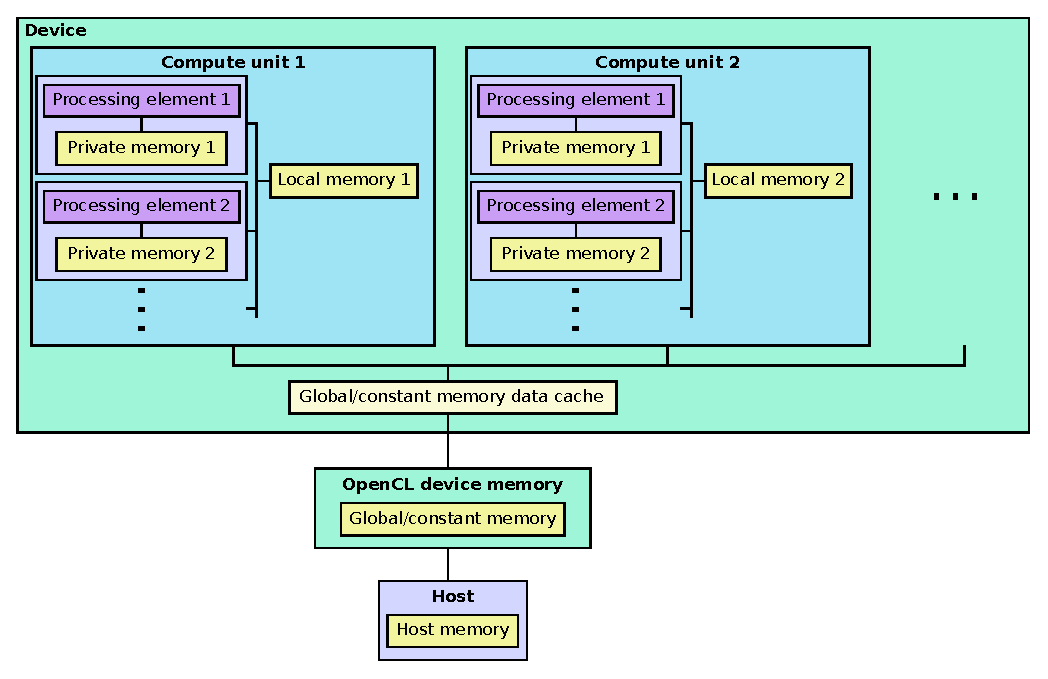
\includegraphics[width=15cm]{images/opencl_memory_model}
\caption{Ein Überblick über die verschiedenen Speicherbereiche, die OpenCL vorgibt, und der Zusammenhang mit dem Execution-Model.}
\label{fig:opencl_memory_model}
\end{figure}

Es ist außerdem möglich, Speicher zwischen OpenGL und OpenCL zu
teilen, sowohl für image-, als auch \PimiddyEnglBegriff{buffer objects}. Dies wird unter
anderem beim Partikelsystem für die Schneeflocken dazu verwendet, die
Eigenschaften der Schneeflocke wie die Position direkt im
OpenGL-Vertexbuffer zu verändern. Es werden so Speicherplatz und
Kopierkosten gespart. Allerdings muss sichergestellt sein, dass alle
OpenCL-Operationen auf dem entsprechenden Buffer abgeschlossen sind,
bevor der Buffer von OpenGL verwendet werden kann. Der umgekehrte
Fall, also der Abschluss aller OpenGL-Operationen auf dem Buffer, muss
auch sichergestellt werden. Dies ist momentan nur möglich, indem man
die Kommandos \PimiddyInlineCode{glFinish} und
\PimiddyInlineCode{clFinish} verwendet. Diese schließen allerdings
global alle noch laufenden Operationen auf \emph{allen} Buffern ab und
blockieren solange das Hauptprogramm. Es kann daher zu
Performanceproblemen kommen.

\subsubsection{OpenCL-C}

In diesem Abschnitt wird die Programmiersprache OpenCL-C eingeführt,
sowie die Zusammenhänge zu den vorher besprochenen Abschnitten
deutlich gemacht. Es soll dabei zunächst der Weg vom fertig
geschriebenen OpenCL-C-Programmtext zu seiner Ausführung auf einem
Device deutlich gemacht werden. Bei den Erklärungen wird
zwischen dem Host-Programm und dem OpenCL-C-Programm hin- und
hergesprungen. Dabei ist zu beachten, dass die von der OpenCL-Runtime
bereitgestellten Funktionen immer mit
\PimiddyQuotes{\PimiddyInlineCode{cl}} beginnen. Diese Funktionen
werden also immer auf dem Host ausgeführt. Im Anschluss werden
einige Besonderheiten von OpenCL-C gegenüber C99 herausgestellt.

OpenCL-C ist momentan die einzige Programmiersprache, welche die
OpenCL-Spe\-zi\-fi\-ka\-ti\-on zur Erstellung von OpenCL-Kerneln formal
beschreibt. Sie basiert auf der ISO-genormten Sprache C99 (genauer
ISO/IEC 9899:1999), wobei einige sprachliche Erweiterungen und eine
große Standardbibliothek ergänzt wurden. Im Folgenden wird minimales
Grundwissen über C99 vorausgesetzt.

OpenCL-C-Programme werden entweder in separaten Textdateien
gespeichert und im Host-Programm in einen String geladen, oder sie
werden direkt im Host-Programm als Stringliteral eingebunden. Der
String mit dem Programmcode wird dann für ein bestimmtes
Device\PimiddyFootnote{Streng genommen ist es eine Liste von Devices.}
mit Hilfe der Funktionen \PimiddyInlineCode{clCreateProgramWithSource}
und \PimiddyInlineCode{clBuildProgram} kompiliert und es entsteht ein
\PimiddyBegriff{program object}. Beim Kompilieren lassen sich noch
Optimierungsflags angeben. Ein Beispiel soll die folgenden Erklärungen
verdeutlichen:

\begin{minted}[frame=lines]{c}
// Hilfsfunktion zum Quadrieren eines Werts.
// Achtung: Nicht von aussen aufrufbar!
float square(float x)
{
  return x*x;
}

// Quadriert ein Array und addiert eine Konstante.
kernel void square_and_add(
    global float *a,
    private float b)
{
  private float current_value = a[get_global_id(0)];
  a[get_global_id(0)] = helper(current_value) + b;
}

constant float4 null_value = (float4)(0.0f);

// Setzt alle Pixel eines 2D-Bildes auf 0 zurueck.
kernel void null_image(
    global write_only image2d_t bild)
{
  write_imagef(
    bild,
    (int2)(
        get_global_id(0),
        get_global_id(1)),
    (float4)(
        0.0f));
}
\end{minted}

Aus dem \PimiddyEnglBegriff{program object} lassen sich nun mittels
\PimiddyInlineCode{clCreateKernel} ein oder mehrere
\PimiddyBegriff{kernel object} erzeugen. In OpenCL-C sind Kernel
normale C99-Funktionen mit Rückgabetyp \PimiddyInlineCode{void}, die
mit dem Attribut \PimiddyInlineCode{kernel} ausgestattet sind. Nur
diese Funktionen können von außen als \PimiddyQuotes{Einsprungpunkte}
für die OpenCL-Runtime benutzt werden. Aus der Funktion
\PimiddyInlineCode{helper} im Programmcode oben kann \PimiddyzB kein
\PimiddyEnglBegriff{kernel object} erzeugt werden. Die Funktion
\PimiddyInlineCode{clCreateKernel} erhält das \PimiddyEnglBegriff{program object} und den
Namen des Kernels als Parameter.

Die Kernelfunktionen in OpenCL-C erhalten Parameter, die vom
Host-Programm vor der Ausführung des Kernels gesetzt werden
müssen. Die Funktion \PimiddyInlineCode{clSetKernelArg} erhält dazu das
\PimiddyEnglBegriff{kernel object}, den Index des Parameters, den man setzen will, sowie den
Parameter selber.

\PimiddyEnglBegriff{Buffer objects} werden in OpenCL-C als \emph{Pointer} repräsentiert. Die
Sprache sieht keine mehrdimensionalen Strukturen vor. Diese müssen
mittels Indextransformationen selber geschrieben werden. \PimiddyEnglBegriff{Image objects}
haben den speziellen Typ \PimiddyInlineCode{image2d\_t}
bzw. \PimiddyInlineCode{image3d\_t} und müssen mit
\PimiddyInlineCode{read\_only} bzw. \PimiddyInlineCode{write\_only}
qualifiziert werden (gleichzeitiger Lese-, und Schreibzugriff ist
aufgrund von Hardwarebeschränkungen nicht möglich). Zum Schreiben
steht die Funktion \PimiddyInlineCode{write\_imagef}, zum Lesen die
Funktion \PimiddyInlineCode{read\_imagef} zur Verfügung.

Sind alle Parameter gesetzt, kann man der Funktion
\PimiddyInlineCode{clEnqueueNDRangeKernel} das \PimiddyEnglBegriff{kernel object}, sowie die
in \autoref{sec:opencl_execution_model} beschriebenen Parameter
übergeben und der Kernel wird auf dem Device ausgeführt.

In OpenCL ist es wichtig, jede Variable mit einem Attribut
auszustatten, die den Speicherbereich der Variable angibt. Mit
Ausnahme des Hostspeichers gibt es für jeden der in
\autoref{sec:opencl_memory_model} beschriebenen Bereiche ein
Schlüsselwort: \PimiddyInlineCode{private},
\PimiddyInlineCode{constant}, \PimiddyInlineCode{local} und
\PimiddyInlineCode{global}. Schreibt man den Speicherbereich nicht
explizit hin, wird \PimiddyInlineCode{private}
angenommen. Speicherbereiche dürfen nicht gemischt werden. So ist es
nicht möglich, einem \PimiddyInlineCode{global float *p} einen Pointer
\PimiddyInlineCode{local float *u} zuzuweisen.

OpenCL-C definiert neue Datentypen für Vektoren. Diese heißen genauso
wie die skalaren Typen in C und haben ihre Dimension angehängt
(\PimiddyzB \PimiddyInlineCode{float4} im Beispiel oben). Für die
Dimension sind allerdings nur $1,2,4,8$ und $16$ möglich. Mit
OpenCL-1.1 ist die Dimension $3$ hinzugekommen. Für Vektoren sind die
arithmetischen Operatoren in natürlicher Weise überladen, sodass man
zwei Vektoren beispielsweise einfach mit \PimiddyInlineCode{a+b}
addieren kann. Vektorliterale sind von der Form
\PimiddyInlineCode{(Typ)(a,b,c,\ldots)}. Als Kurzform steht auch
\PimiddyInlineCode{(Typ)(a)} zur Verfügung, was den kompletten Vektor
mit dem Wert \PimiddyInlineCode{a} initialisiert. Auf diese Form der
Initialisierung wird in der Implementierung häufiger
zurückgegriffen. Auf die einzelnen Komponenten eines Vektors kann man
mit dem \PimiddyInlineCode{.}-Operator wie auf die Komponenten einer
Struktur zugreifen, also z.B. \PimiddyInlineCode{v.x}.

OpenCL-C bietet außerdem eine umfangreiche Standardbibliothek. Sie
enthält vor allem mathematische Funktionen, die allerdings auch für
die Vektortypen überladen sind. Die Funktion \PimiddyInlineCode{sin}
zur Berechnung des Sinus steht beispielsweise auch für Vektoren zur
Verfügung und arbeitet dort komponentenweise. Auch
\PimiddyQuotes{echte} Vektorfunktionen wie das Kreuz-, und das
Skalarprodukt (\PimiddyInlineCode{cross}, \PimiddyInlineCode{dot})
stehen zur Verfügung und können auf manchen Systemen in schnelle
SIMD-Instruktionen übersetzt werden. Die verwendeten
Bibliotheksfunktionen werden in der Implementierung an passender
Stelle erklärt, statt sie hier komplett aufzuführen.

Die Sprache listet allerdings einige Einschränkungen, damit sie auch
auf minimalen Prozessoren lauffähig ist:

\begin{itemize}
\item Rekursive Funktionen sind nicht erlaubt.
\item Funktionspointer sind nicht erlaubt.
\item Pointer auf Pointer sind zwar erlaubt, aber nicht als Kernelparameter.
\item Dynamische Speicherverwaltung (normalerweise mit Hilfe der Funktionen \PimiddyInlineCode{malloc} und \PimiddyInlineCode{free}) ist nicht vorgesehen.
\item Die C-Standardbibliothek steht nicht zur Verfügung.
\end{itemize}

\subsection{Beispielcode}

Um das Zusammenspiel aller OpenCL-Komponenten zu verdeutlichen, soll
hier der Programmcode vorgestellt werden, um zwei Arrays einzulesen,
sie mit \PimiddyListingRef{lst:opencl_add_arrays_example} zu addieren
und das Ergebnis auszugeben. Es wird leicht vereinfachter C-Code
verwendet und \PimiddyzB Fehlerbehandlung weggelassen.

Wir nehmen an, die Variable \PimiddyInlineCode{device} enthielte das
Gerät, auf dem der Code ausgeführt werden soll. Außerdem sei die Länge
der Arrays auf 100 festgelegt. Das Host-Programm beginnt damit, die
nötigen \PimiddyEnglBegriff{buffer objects} zu erstellen:

\begin{minted}[frame=lines]{c}
// Diese beiden Arrays koennten vom Benutzer auf der
// Kommandozeile eingelesen werden
float erstes_array[100],zweites_array[100];

cl_mem a = clCreateBuffer(
    device,
    CL_MEM_READ_ONLY,
    100 * sizeof(float),
    erstes_array);

cl_mem b = clCreateBuffer(
    device,
    CL_MEM_READ_ONLY,
    100 * sizeof(float),
    zweites_array);

cl_mem result = clCreateBuffer(
    device,
    CL_MEM_READ_WRITE,
    100 * sizeof(float),
    // Der Inhalt dieses Buffers wird nicht vorgegeben.
    NULL);
\end{minted}

Wie bereits angesprochen, erhält die Funktion \PimiddyInlineCode{clCreateBuffer}
die Größe des Buffers in Bytes (daher das \PimiddyInlineCode{sizeof(float)}) und
zudem ein Flag, welches angibt, ob der Buffer nur gelesen
(\PimiddyInlineCode{CL\_MEM\_READ\_ONLY}) oder auch geschrieben werden kann
(\PimiddyInlineCode{CL\_MEM\_READ\_WRITE}). Die Buffer, die als Eingabe für den
Algorithmus dienen, werden direkt mit den vom Benutzer vorgegebenen Arrays
gefüllt und sind im weiteren nur lesbar. Der \PimiddyInlineCode{result}-Buffer
bleibt uninitialisiert (es wird \PimiddyInlineCode{NULL} als Inhalt übergeben),
denn es wird vom Kernel gefüllt. \PimiddyInlineCode{clCreateBuffer} liefert ein
Handle vom Typ \PimiddyInlineCode{cl\_mem} zurück, welches an andere Funktionen
weitergereicht werden kann.

Danach wird das \PimiddyEnglBegriff{program object} aus dem Quellcode erstellt
und kompiliert. Das zurückgegebene \PimiddyInlineCode{cl\_program}-handle kann
dann zur Erstellung eines \PimiddyEnglBegriff{kernel object} verwendet werden.
Es wird angenommen, dass der Quelltext des Programms in einem String
\PimiddyInlineCode{program\_source\_code} gespeichert ist:

\begin{minted}[frame=lines]{c}
cl_program program = clCreateProgramWithSource(
    device,
    program_source_code);

clBuildProgram(
    program,
    // Optionale Parameter fuer den Compiler
    "");

cl_kernel kernel = clCreateKernel(
    program,
    "add_arrays");
\end{minted}

Das so konstruierten \PimiddyInlineCode{cl\_kernel}-Handle können nun mittels
der Funktion \PimiddyInlineCode{clSetKernelArg} die Buffer übergeben werden. Die
OpenCL-Runtime unterstützt die Zuweisung von Kernelparametern nur mittels Index,
nicht via Name:

\begin{minted}[frame=lines]{c}
clSetKernelArg(
    kernel,
    0,
    a);
clSetKernelArg(
    kernel,
    1,
    b);
clSetKernelArg(
    kernel,
    2,
    result);
\end{minted}

Das Programm ist jetzt bereit zur Ausführung:

\begin{minted}[frame=lines]{c}
clEnqueueNDRangeKernel(
    device,
    kernel,
    // Globale Arbeitsgroesse
    100,
    // Keine lokale Arbeitsgroesse
    NULL);
\end{minted}

Wenn die Funktion zurückgibt, hat das Device seine Arbeit verrichtet und das
Ergebnis liegt in \PimiddyInlineCode{result}. Dieses \PimiddyEnglBegriff{buffer
object} liegt allerdings im globalen Device-Speicher. Um die Werte
\PimiddyzB auf der Konsole auszugeben, wird der Inhalt in den
Host-Speicher übertragen.

\begin{minted}[frame=lines]{c}
float result_host_memory[100];

float *result_array = clEnqueueMapBuffer(
    result);

copy(result_array,result_host_memory);

clEnqueueUnmapBuffer(
    result);
\end{minted}

Die Variable \PimiddyInlineCode{result\_host\_memory} enthält jetzt
$a+b$, wobei komponentenweise addiert wurde.
